\documentclass[11pt, oneside]{article} 
\usepackage{geometry}
\geometry{letterpaper} 
\usepackage{graphicx}
	
\usepackage{amssymb}
\usepackage{amsmath}
\usepackage{parskip}
\usepackage{color}
\usepackage{hyperref}

\graphicspath{{/Users/telliott_admin/Dropbox/Tex/png/}}
% \begin{center} 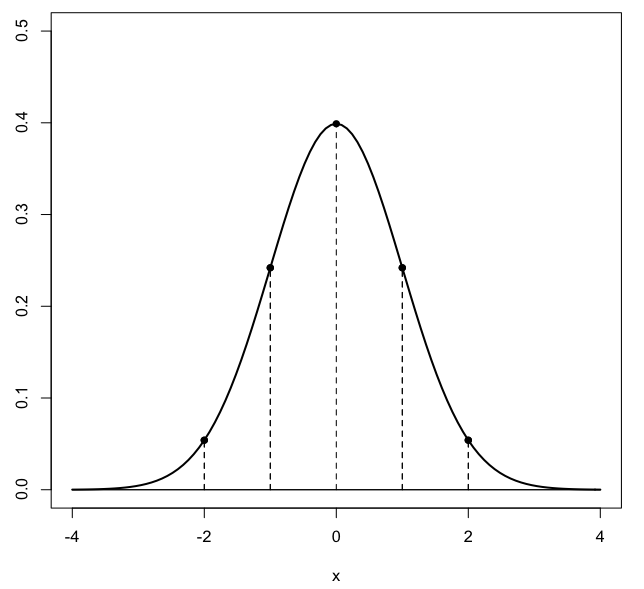
\includegraphics [scale=0.4] {gauss3.png} \end{center}

\title{Heron's Formula}
\date{}

\begin{document}
\maketitle
\Large

Heron's Formula can be used to compute the area of a triangle from the lengths of its sides.  It is a simple formula that does not explicitly include the altitude $h$ or the parts of side $c$.
\begin{center}
\includegraphics [scale=0.5] {triangle.png}
\end{center}

If $s$ is the semi-perimeter
\[ s = \frac{1}{2}(a + b + c) \]
then
\[ A = \sqrt{s + (s-a) + (s-b) + (s-c)} \]

\subsection*{Lockhart's version}
\begin{center} 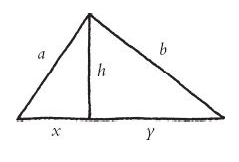
\includegraphics [scale=0.5] {triangle2.png} \end{center}
Here the triangle is labeled slightly differently than the one above.  The bottom side $c$ is split into $x$ and $y$.  We can write three equations:

\[ x^2 + h^2 = a^2 \]
\[ y^2 + h^2 = b^2 \]
\[ x + y = c \]

Our ultimate objective is an equation that contains only $a$, $b$ and $c$. Lockhart gives us a target for the first part of the derivation:

\[ 2xc = c^2 + a^2 - b^2 \]

Let's just start manipulating equations to get there.  Subtract the second from the first:
\[ x^2 - y^2 = a^2 - b^2 \]
Square the third
\[ x^2 + 2xy + y^2 = c^2 \]

Add the two new equations
\[ 2x^2 + 2xy =  c^2 + a^2 - b^2 \]

Substitute for $y$
\[ 2x^2 + 2x(c-x) =  c^2 + a^2 - b^2 \]
\[ 2xc = c^2 + a^2 - b^2  \]

Finally a slight rearrangement:
\[ x = \frac{c^2 + a^2-b^2}{2c} = \frac{c}{2} + \frac{a^2-b^2}{2c}   \]

This says that to find the point where $c$ is divided into $x$ and $y$, we move from the center $c/2$ a distance of $(a^2 - b^2)/2c$.

The corresponding equation for $y$ is
\[ y = \frac{c}{2} - \frac{a^2-b^2}{2c} \]
which is easily checked by adding together the final two equations, obtaining $x + y = c$.

For the area, we will need $h$ somehow.  It is easier to use $h^2$.
\[ h^2 = a^2 - x^2 \]
\[ = a^2 - \frac{(c^2 + a^2-b^2)^2}{(2c)^2}  \]

The area squared is
\[ A^2 = \frac{1}{4}c^2 h^2 \]
\[ = \frac{1}{4} c^2 a^2 - \frac{1}{4} c^2 \frac{(c^2 + a^2-b^2)^2}{(2c)^2}  \]

Lockhart:

\begin{quote}
the algebraic form of this measurement is aesthetically unacceptable. First of all, it is not symmetrical; second, it's hideous. I simply refuse to believe that something as natural as the area of a triangle should depend on the sides in such an absurd way. It must be possible to rewrite this ridiculous expression...
\end{quote}

Here's a start:
\[ 16A^2 = (2ac)^2 - (c^2 + a^2-b^2)^2 \]

This is much better, notice that we have only $a$, $b$ and $c$.

We will now go through two difference of squares manipulations.  First

\[ 16A^2 = \ [ \ 2ac + (c^2 + a^2-b^2) \ ] \ [ \ 2ac - (c^2 + a^2-b^2) \ ]  \]
\[ = \ [ \ (a + c)^2 -b^2) \ ] \ [ \ b^2 - (a - c)^2 \ ]  \]
\[ =  (a + c + b)(a + c - b)(b + a - c)(b - a + c) \]
So
\[ A = \sqrt{\frac{a + b + c}{2}  \cdot \frac{a + c - b}{2}  \cdot \frac{a + b - c}{2}  \cdot \frac{-a + b + c}{2} } \]

At this point, we recognize the semi-perimeter $s = (a + b + c)/2$ and then we see that each of the other terms is $s$ minus one of the sides
\[ A = \sqrt{s \cdot (s - a) \cdot (s - b) \cdot (s - c) } \]
\subsection*{check}
As a simple example, if we have a right triangle with sides 3,4,5, then the area is one-half of 3 times 4 = 6.  The semi-perimeter is s

\[ s = \frac{(3 + 4 + 5)}{2} = \frac{12}{2} = 6 \]
We have

\[ A =  \sqrt { 6 (6-5) (6-4) (6-3) } =  \sqrt { 6 (1) (2) (3) } = 6 \]


\end{document}  